In this chapter the different models used in this thesis are described. The loop expansion, giving the context of the Worm algorithm is examined for each model. The method of determining the critical temperature of an XY lattice using the winding number is discussed.

Finally the definition of the Hausdorff dimension is shown and different ways of determining it is discussed.

\section{Ising model}

The Ising model consists of discrete atomic spins $S$ that can be found in two states represented by the values $\{-1, 1\}$. This can be applied to a lattice where $S_i$ is the spin of lattice site $i$.

The energy of such a configuration is then given by the Hamiltonian

\begin{equation}
    H = - J \sum_{\langle ij \rangle} S_i S_j
\label{eq:isingmodelhamiltonian}
\end{equation}

where $J$ is the bond strength in the lattice and $\langle ij \rangle$ refers to an only nearest neighbour interaction.

\subsection{Loop expansion}
\label{subsec:IsingLoopExpansion}

Let $K = \beta J$ where $\beta = 1/k_{\text{B}} T$. Then from Equation (\ref{eq:isingmodelhamiltonian})

\begin{equation}
    \beta E = - K \sum_{\langle ij \rangle} S_i S_j
\end{equation}

The partition function $Z$ can therefore be written as

\begin{equation}
    Z = \sum_{\text{all states}} e^{-\beta E} = \sum_{\text{all states}} e^{K \sum_{\langle ij \rangle} S_i S_j} = \sum_{\text{all states}} \Pi_{\langle ij \rangle} e^{K S_i S_j}
\label{Eq:partitionIsingWithoutExpansion}
\end{equation}

Since $S_i S_j = \pm 1$, the Euler identities can be used to expand the exponential in Equation (\ref{Eq:partitionIsingWithoutExpansion}).

\begin{align*}
    e^{KS_i S_j} &= \frac{e^K + e^{-K}}{2} + S_i S_j \frac{e^K - e^{-K}}{2} \\
    &= \cosh (K) + S_i S_j \sinh(K) \\
    &= \{ T = \tanh(K) \} \\
    &= (1 + T S_i S_j) \cosh(K)
\end{align*}

In a $2D$ lattice with $N$ spins and periodic boundary conditions there are $2N$ bonds between sites. Therefore the partition function is

\begin{align*}
    Z &= \sum_{\text{all states}} \Pi_{\langle ij \rangle} (1 + T S_i S_j) \cosh(K) \\
    &= \cosh^{2N} (K) \cdot 2^N \left ( 2^{-N} \sum_{\text{all states}} \Pi_{\langle ij \rangle} (1 + T S_i S_j) \right ) \\
    &= \cosh^{2N} (K) \cdot 2^N Z'
\end{align*}

where

\begin{align*}
    Z' &= 2^{-N} \sum_{\text{all states}} \Pi_{\langle ij \rangle} (1 + T S_i S_j) \\
    &= 2^{-N} \sum_{S_1 = \pm 1} \sum_{S_2 = \pm 1} \ldots \sum_{S_N = \pm 1} \left ( 1 + T \sum_{l = 1} S_i S_j + T^2 \sum_{l = 2} (S_i S_j)(S_{i'} S_{j'}) + \ldots \right ) 
\end{align*}

where the sums $\sum_{l=L}$ should be interpreted as the sum over all sets where the link length is $L$. Link length is the number of coupling terms $S_i S_j$ as can be seen in Figure (\ref{fig:LinkIsing}).

\begin{figure}[h!]
    \begin{subfigure}{.5\linewidth}
        \centering
        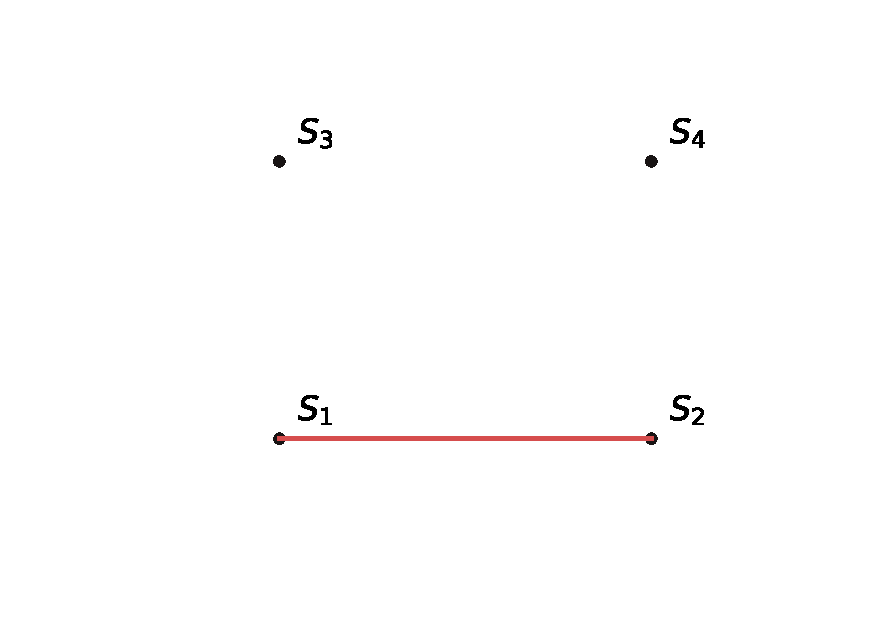
\includegraphics[width=\textwidth]{figures/ising_loop_one_link.pdf}
        \caption{$(S_1 S_2), \ L = 1$}
        \label{fig:oneLinkIsing}
    \end{subfigure}%
    \begin{subfigure}{.5\linewidth}
        \centering
        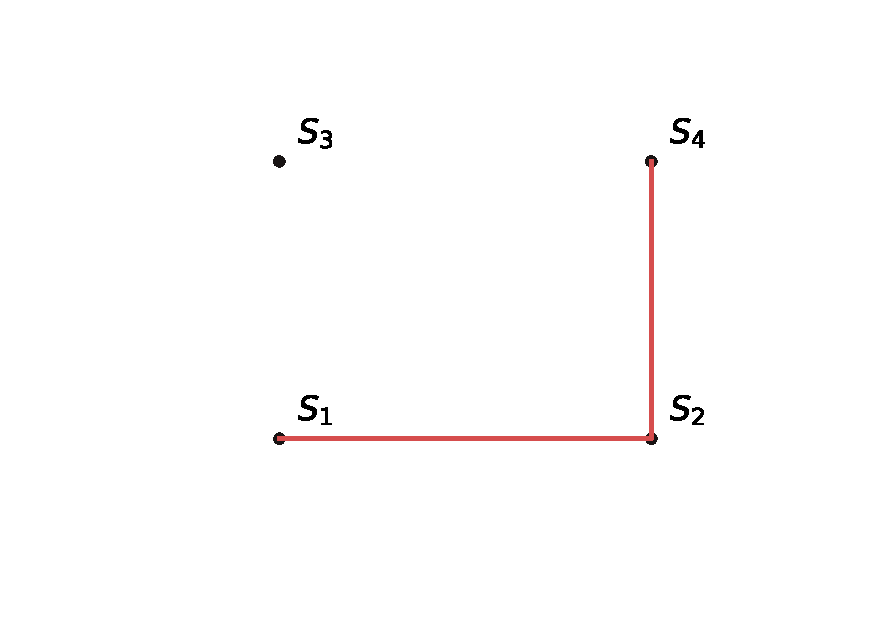
\includegraphics[width=\textwidth]{figures/ising_loop_two_link.pdf}
        \caption{$(S_1 S_2)(S_2 S_4), \ L = 2$}
        \label{fig:twoLinkIsing}
    \end{subfigure}\\[1ex]
    \begin{subfigure}{\linewidth}
        \centering
        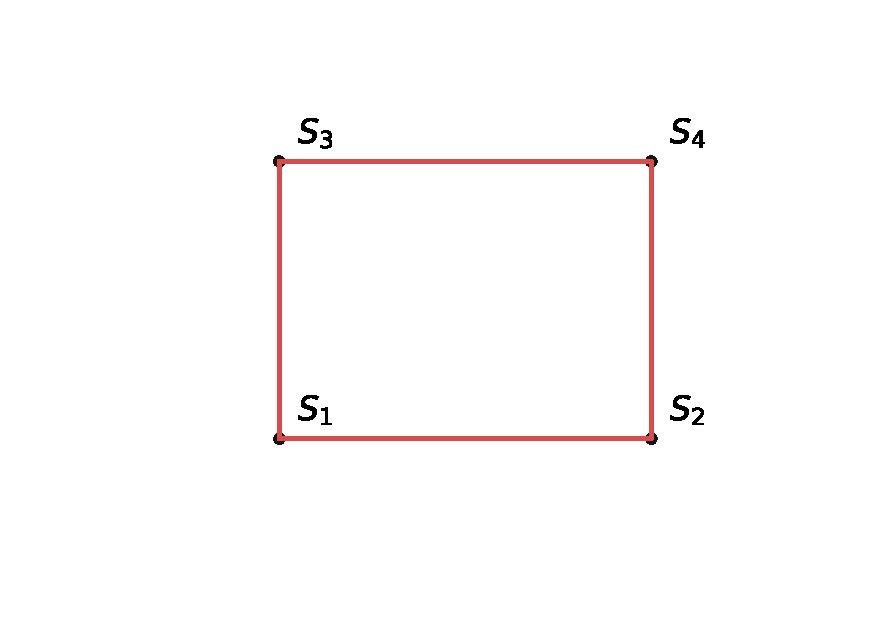
\includegraphics[width=.5\textwidth]{figures/ising_loop_four_link.pdf}
        \caption{$(S_1 S_2)(S_2 S_4)(S_4 S_3)(S_3 S_1), \ L = 4$}
    \label{fig:fourLinkIsing}
    \end{subfigure}
    \caption{Link structure of an Ising lattice where (a) and (b) are open while (c) is closed.}
    \label{fig:LinkIsing}
\end{figure}

Since $\sum_{S_i = \pm 1} S_i = 0$, only terms with an even number of $S_i$ are contributing to $Z'$. Call these terms closed, indicating that they represent a closed loop. The sum over all contributing terms gives a factor of $2^N$.

Rewriting $Z'$ in terms of loop lengths gives

\begin{equation}
    Z' = \sum_L g(L) T^L
\end{equation}

where $g(L)$ is the number of loops with length $L$. Finally, the partition function can be written as

\begin{equation}
    Z = 2^N \cosh^{2N} (K) \sum_L g(L) T^L
\end{equation}

\subsection{Correlation Function}
\label{subsec:CorrelationFunction}

By the fluctuation-dissipation theorem the susceptibility can be written as 

\begin{equation}
    \chi = \frac{\beta}{N} \sum_{ij} G_{ij}
\end{equation}

where $G_{ij} = \langle S_i S_j \rangle - \langle S_i \rangle^2$ is the connected correlation function between two lattice points $i$ and $j$ \cite{Chaikin:PrincCondencedMatterPhysics}.

In the high-temperature expansion the term $\langle S_i \rangle^2$ goes to zero. Thus, for a $2D$ Ising model

\begin{align}
    G_{ij} &= \frac{1}{Z} \sum_{\text{all states}} S_i S_j e^{-\beta E} \\
    &= \left \{ \text{see Section \ref{subsec:IsingLoopExpansion}} \right \} \\
    &= \frac{1}{Z} \cosh^{2N} (K) \sum_{\text{all states}} S_i S_j \Pi_{\langle ij \rangle} (1 + \tanh(K) S_i S_j)
\end{align}

hence, the acceptance probability is \cite{Walter:IntroToMC}

\begin{equation}
A_{ab} = \left\{
\begin{array}{ll}
      \min \left (1, \tanh(K)\right), \ \text{To create a link between $a$ and $b$.} \\
      \min \left (1, \frac{1}{\tanh(K)} \right), \ \text{To remove a link between $a$ and $b$.}
\end{array} 
\right. 
\end{equation}



\section{$n$-vector model}
\label{sec:nVector}

The $n$-vector model describes a classical system of $n$-dimensional classical spins $s_i$ of unit length interacting on a lattice. It is a generalization of the Ising model where each spin can have a continuous set of values. The Hamiltonian is then

\begin{equation}
    H = -J\sum_{\langle ij \rangle} s_i \cdot s_j
\end{equation}

where $J$ is the bond strength and $\langle ij \rangle$ refers to a nearest neighbour interaction.

\section{XY model}
\label{sec:XYModel}

A special case of the $n$-vector model is the XY model when $n = 2$. Here the spins are two dimensional rotors as $s_i = (\cos \theta_i, \  \sin \theta_i)$. This yields the Hamiltonian

\begin{equation}
    H = - J \sum_{\langle ij \rangle} \cos(\theta_i - \theta_j)
\label{eq:xymodel}
\end{equation}

The partition function is therefore

\begin{equation}
    Z = \prod_i \int \frac{\mathrm d \theta_i}{2 \pi} e^{-\beta H} = \prod_i \int \frac{\mathrm d \theta_i}{2 \pi} e^{K \sum_{\langle ij \rangle} \cos(\theta_i - \theta_j)}
\label{eq:xypart1}
\end{equation}

where $K = J \beta$.

\subsection{Loop expansion}
\label{subsec:XYLoopexp}

Since Equation (\ref{eq:xypart1}) is invariant under the transformation $\theta_i - \theta_j \rightarrow \theta_i - \theta_j + 2 \pi n$, $n \in \mathbb{Z}$, it can be expanded using the identity

\begin{equation}
    e^{\alpha \cos \beta} = \sum_{\gamma = -\infty}^{\infty} I_\gamma ( \alpha ) e^{i \gamma \beta}
\end{equation}

where $I_\gamma(\alpha)$ is the modified Bessel function. Using that $e^{\sum_i x_i} = \prod_i e^{x_i}$ gives

\begin{align}
    Z &= \prod_i \int \frac{\mathrm d \theta_i}{2 \pi} \sum_{J_{\langle ij \rangle} = -\infty}^{\infty} \prod_{b = \langle ij \rangle} I_{J_{\langle ij \rangle}} ( K ) e^{i J_{\langle ij \rangle} (\theta_i - \theta_j)} \\
\label{eq:xypart2}
% 
    &=  \prod_i \sum_{J_b} \left ( \int \frac{\mathrm d \theta_i}{2 \pi} e^{i N_i (\theta_i - \theta_j)} \right ) \left ( \prod_b I_{J_b} \right ) 
\end{align}

where in the last step, $\prod_{\langle ij \rangle} e^{iJ_{\langle ij \rangle} (\theta_i - \theta_j)} = e^{iN_i (\theta_i - \theta_j)}$. $N_i$ is therefore the sum of $J$ for the nearest neighbours of site $i$. Noting that

\begin{equation}
    \int \frac{\mathrm d \theta_i}{2 \pi} e^{i N_i (\theta_i - \theta_j)} = C \delta_{N_i 0}
\end{equation}

leads to the conclusion that the sum of incoming and outgoing flux $J$ into a site $i$ must be zero, in other words, the configurations are divergence free. This in turn means that a configuration of the system must contain closed loops of flux $J$.

% NOTE: Explanation to the last sentence; take one site i and impose that it has to be divergence free (some flux out, same flux in). Then impose the same thing on its neighbour. The flux coming out of i must flow into the neighbour. Repeating this process over the whole lattice will give closed loops.

\subsection{Winding number}
\label{subsec:XYWindingNum}

In the ground state all the spins are aligned, while at higher energy states, the spins are pointed in random directions as can be seen in Figure (\ref{fig:xygroundhigher}).

\begin{figure}[h!]
\centering
    \begin{subfigure}{.4\textwidth}
        \centering
        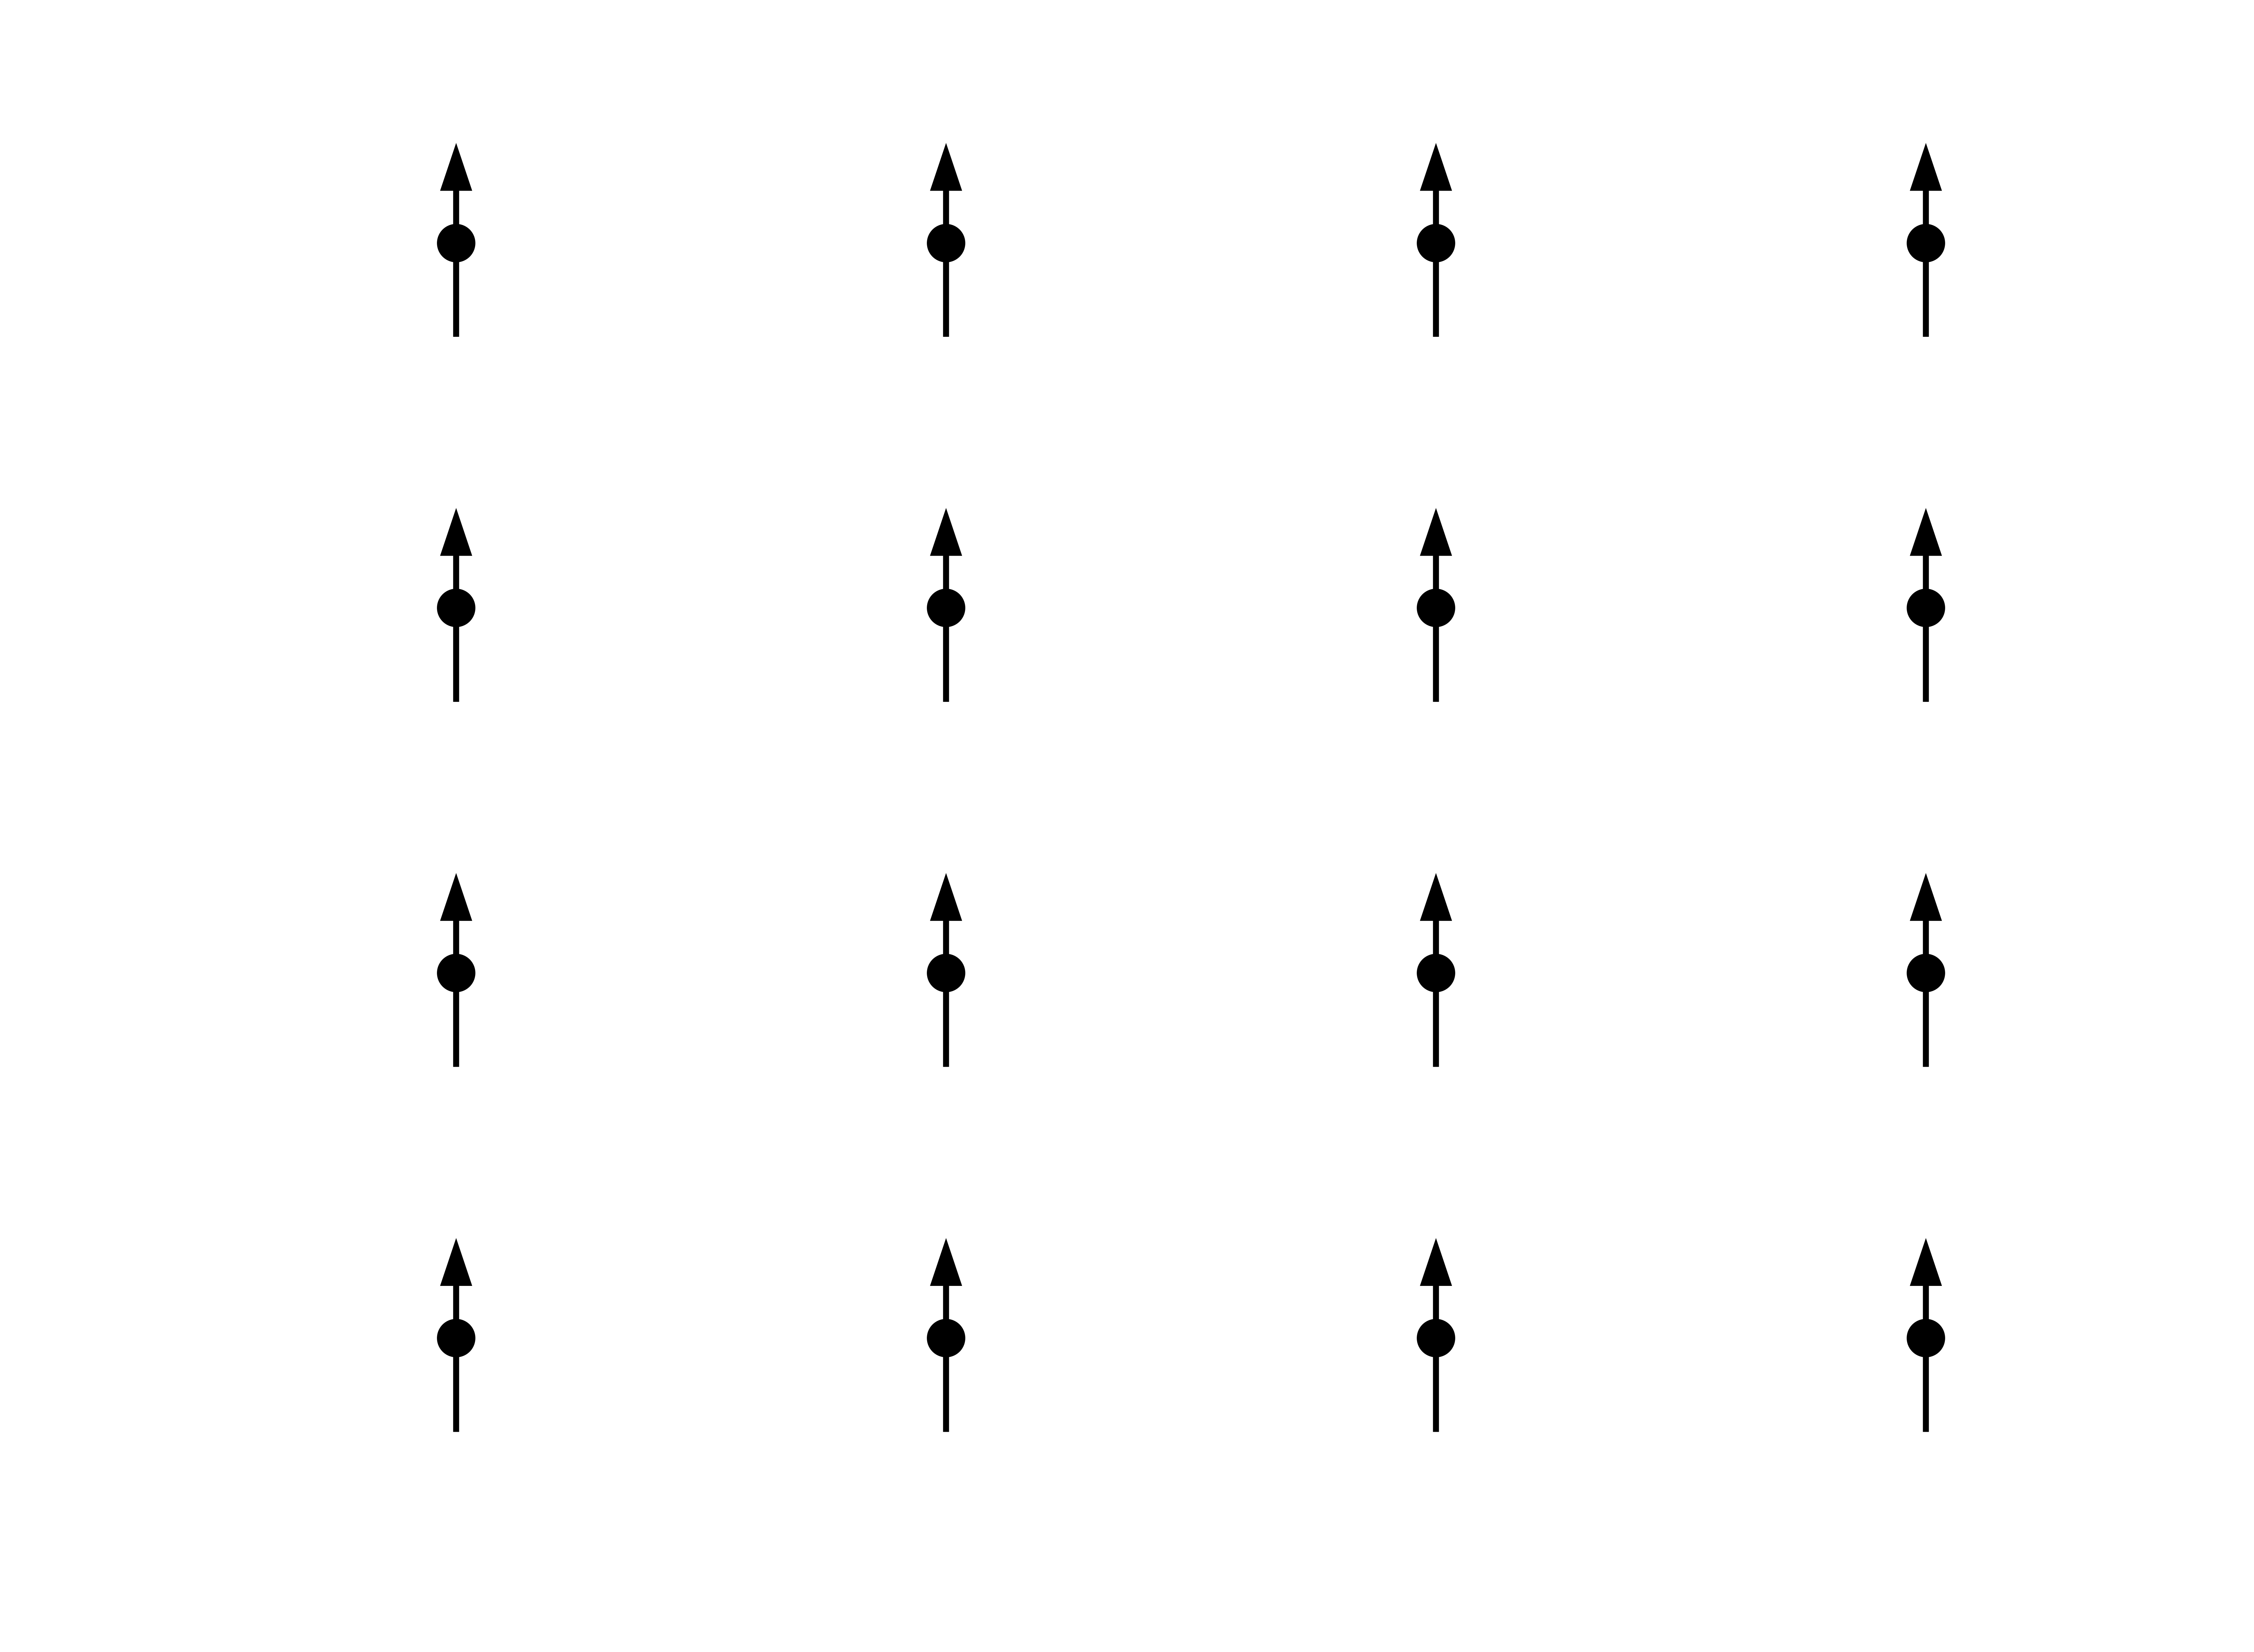
\includegraphics[width=\linewidth]{figures/noPhaseShift.pdf}
        \caption{Ground state}
        \label{fig:xyground}
    \end{subfigure}
    \begin{subfigure}{.4\textwidth}
        \centering
        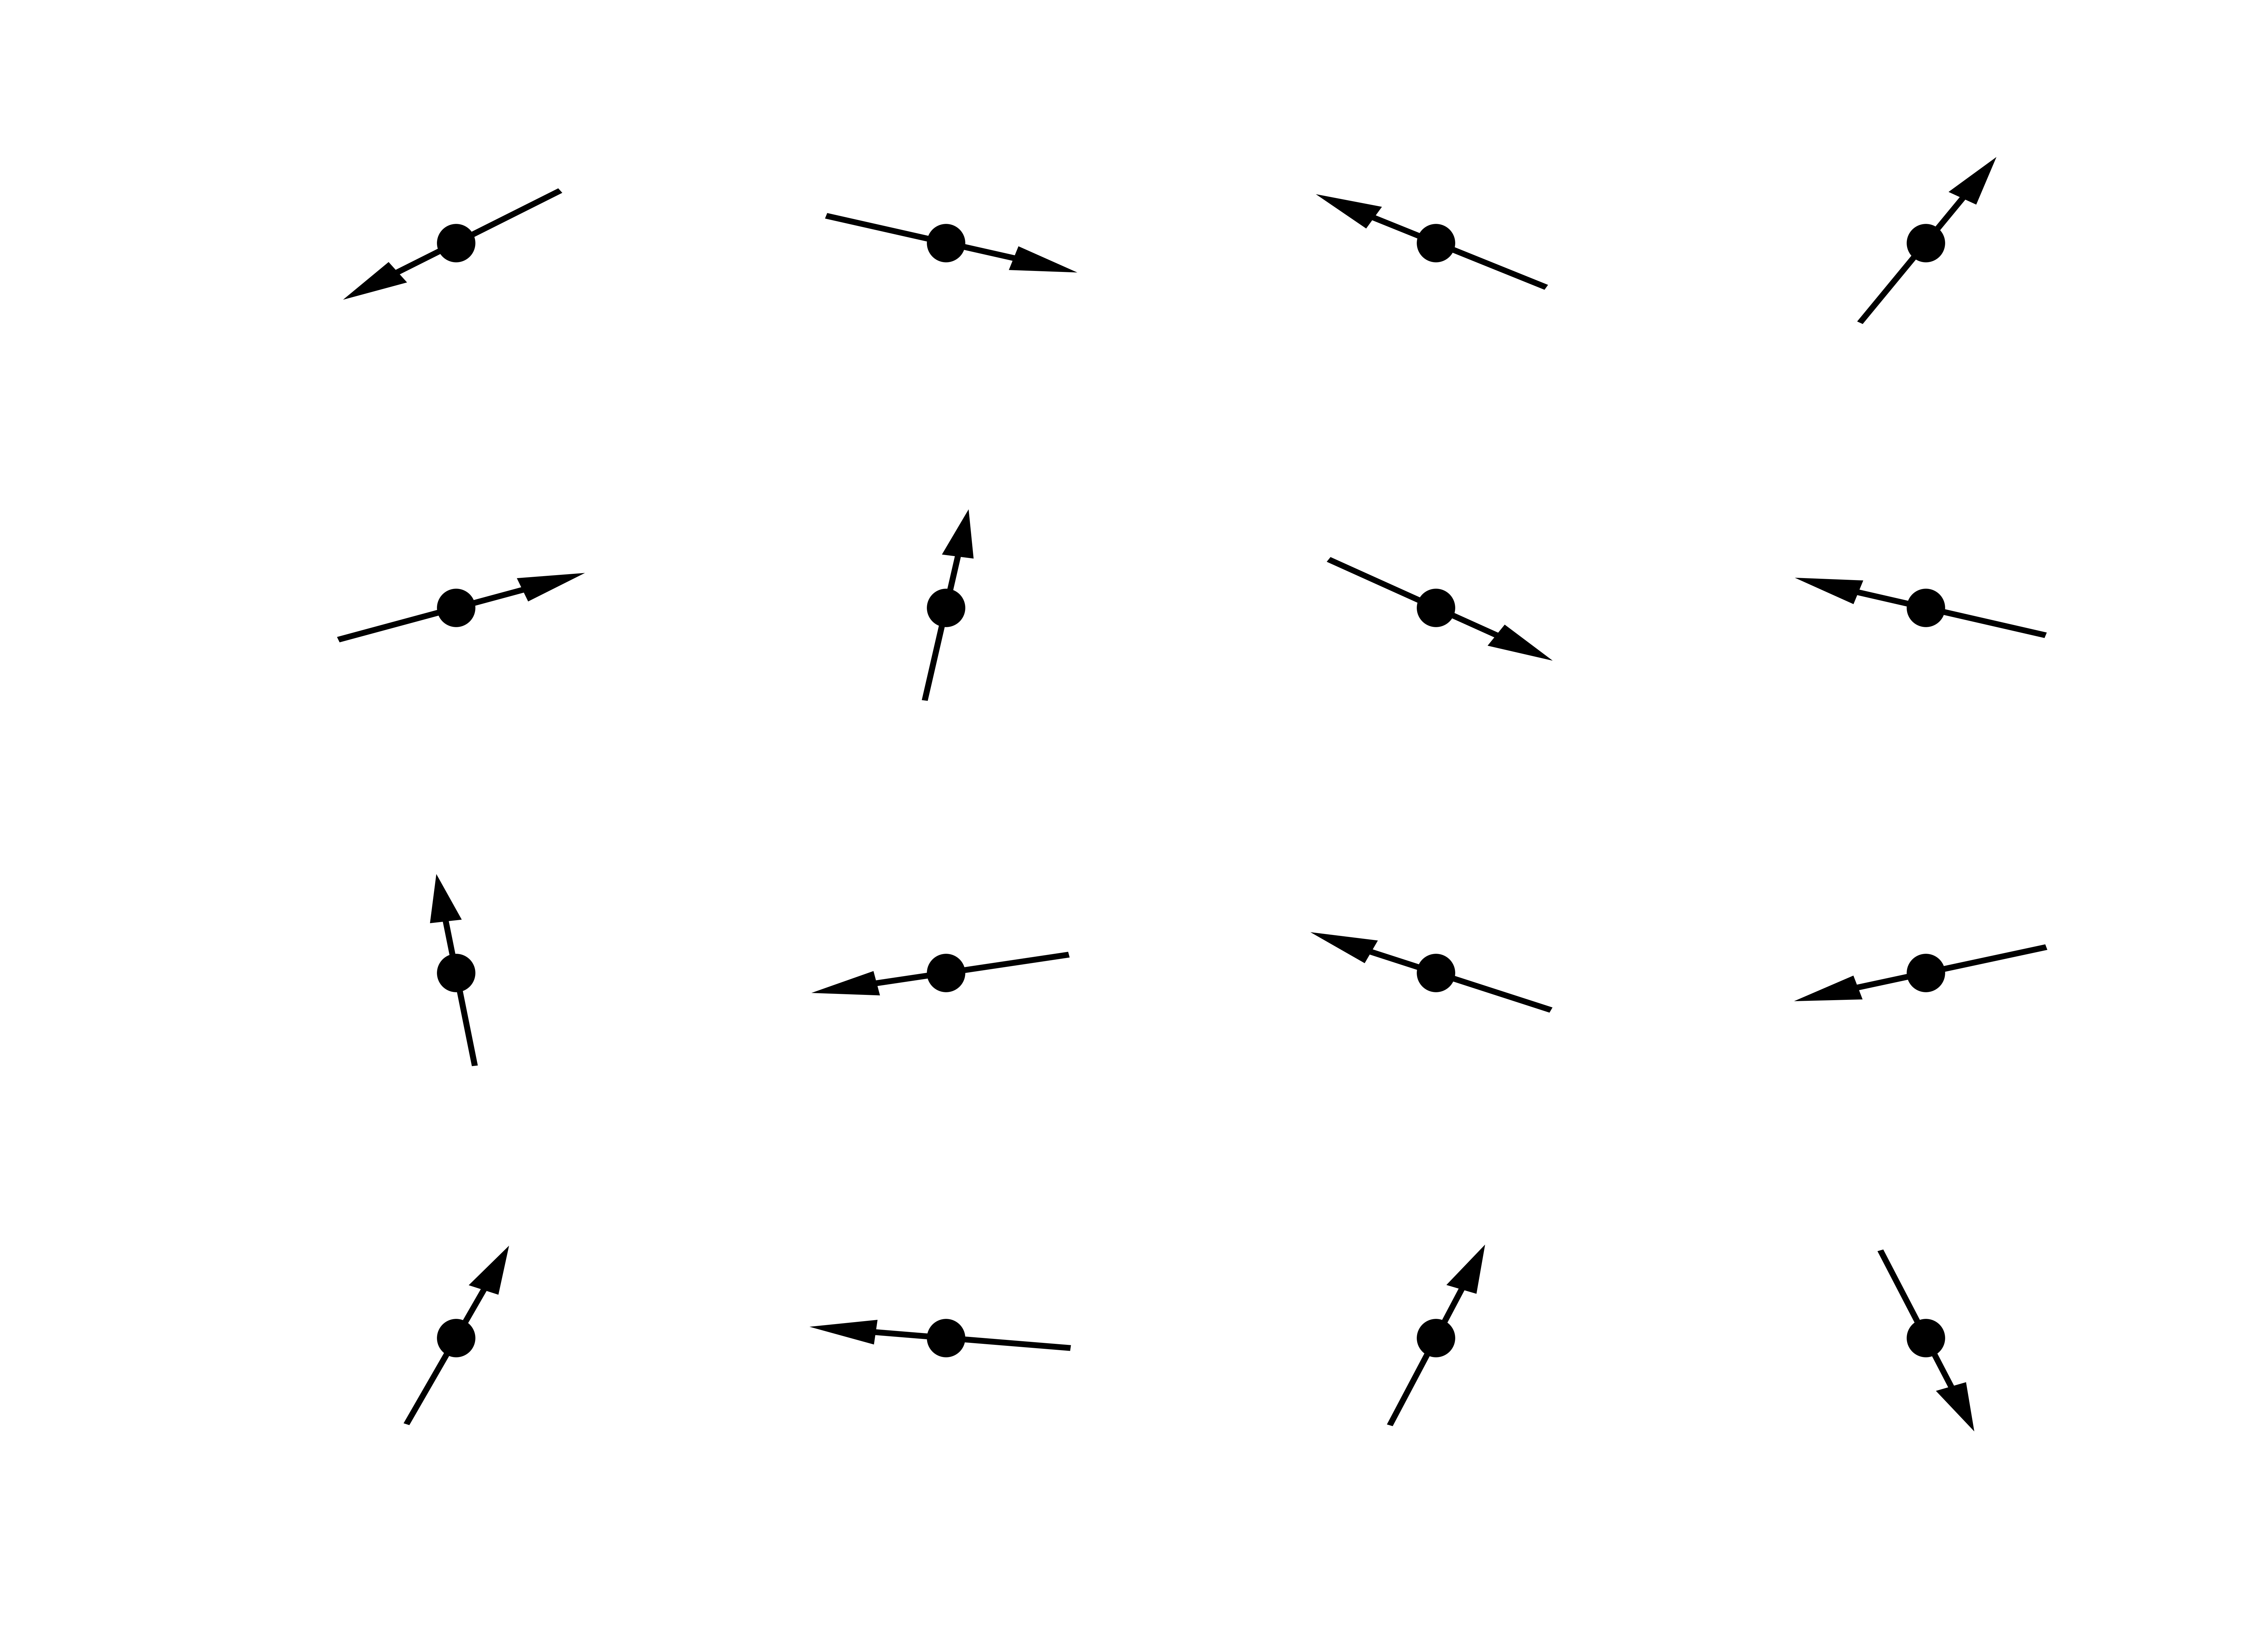
\includegraphics[width=\linewidth]{figures/randomAngle.pdf}
        \caption{Higher energy state}
        \label{fig:xyhigher}
    \end{subfigure}
    \caption{Energy states for XY model}
\label{fig:xygroundhigher}
\end{figure}

Therefore, making a constant phase shift $\Phi_\mu = \frac{A}{L}$ of $\theta_i - \theta_j$ in the $\mu$ direction would change the energy drastically for the ground state while, on a statistical average, not change the higher states energy at all (see Figure (\ref{fig:xyphaseshift})).

\begin{figure}[h!]
\centering
    \begin{subfigure}{.4\textwidth}
        \centering
        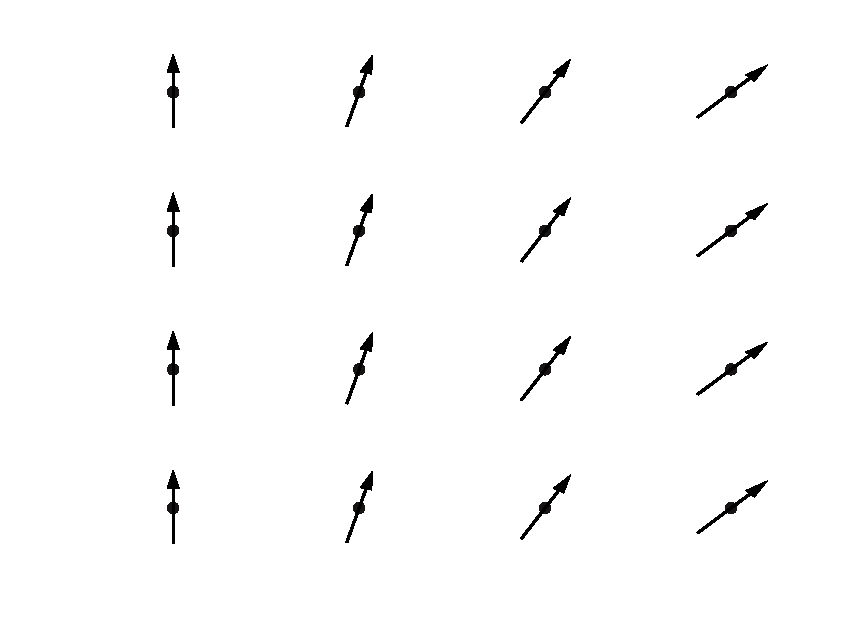
\includegraphics[width=\linewidth]{figures/PhaseShift.pdf}
        \caption{Ground state}
        \label{fig:xyground}
    \end{subfigure}
    \begin{subfigure}{.4\textwidth}
        \centering
        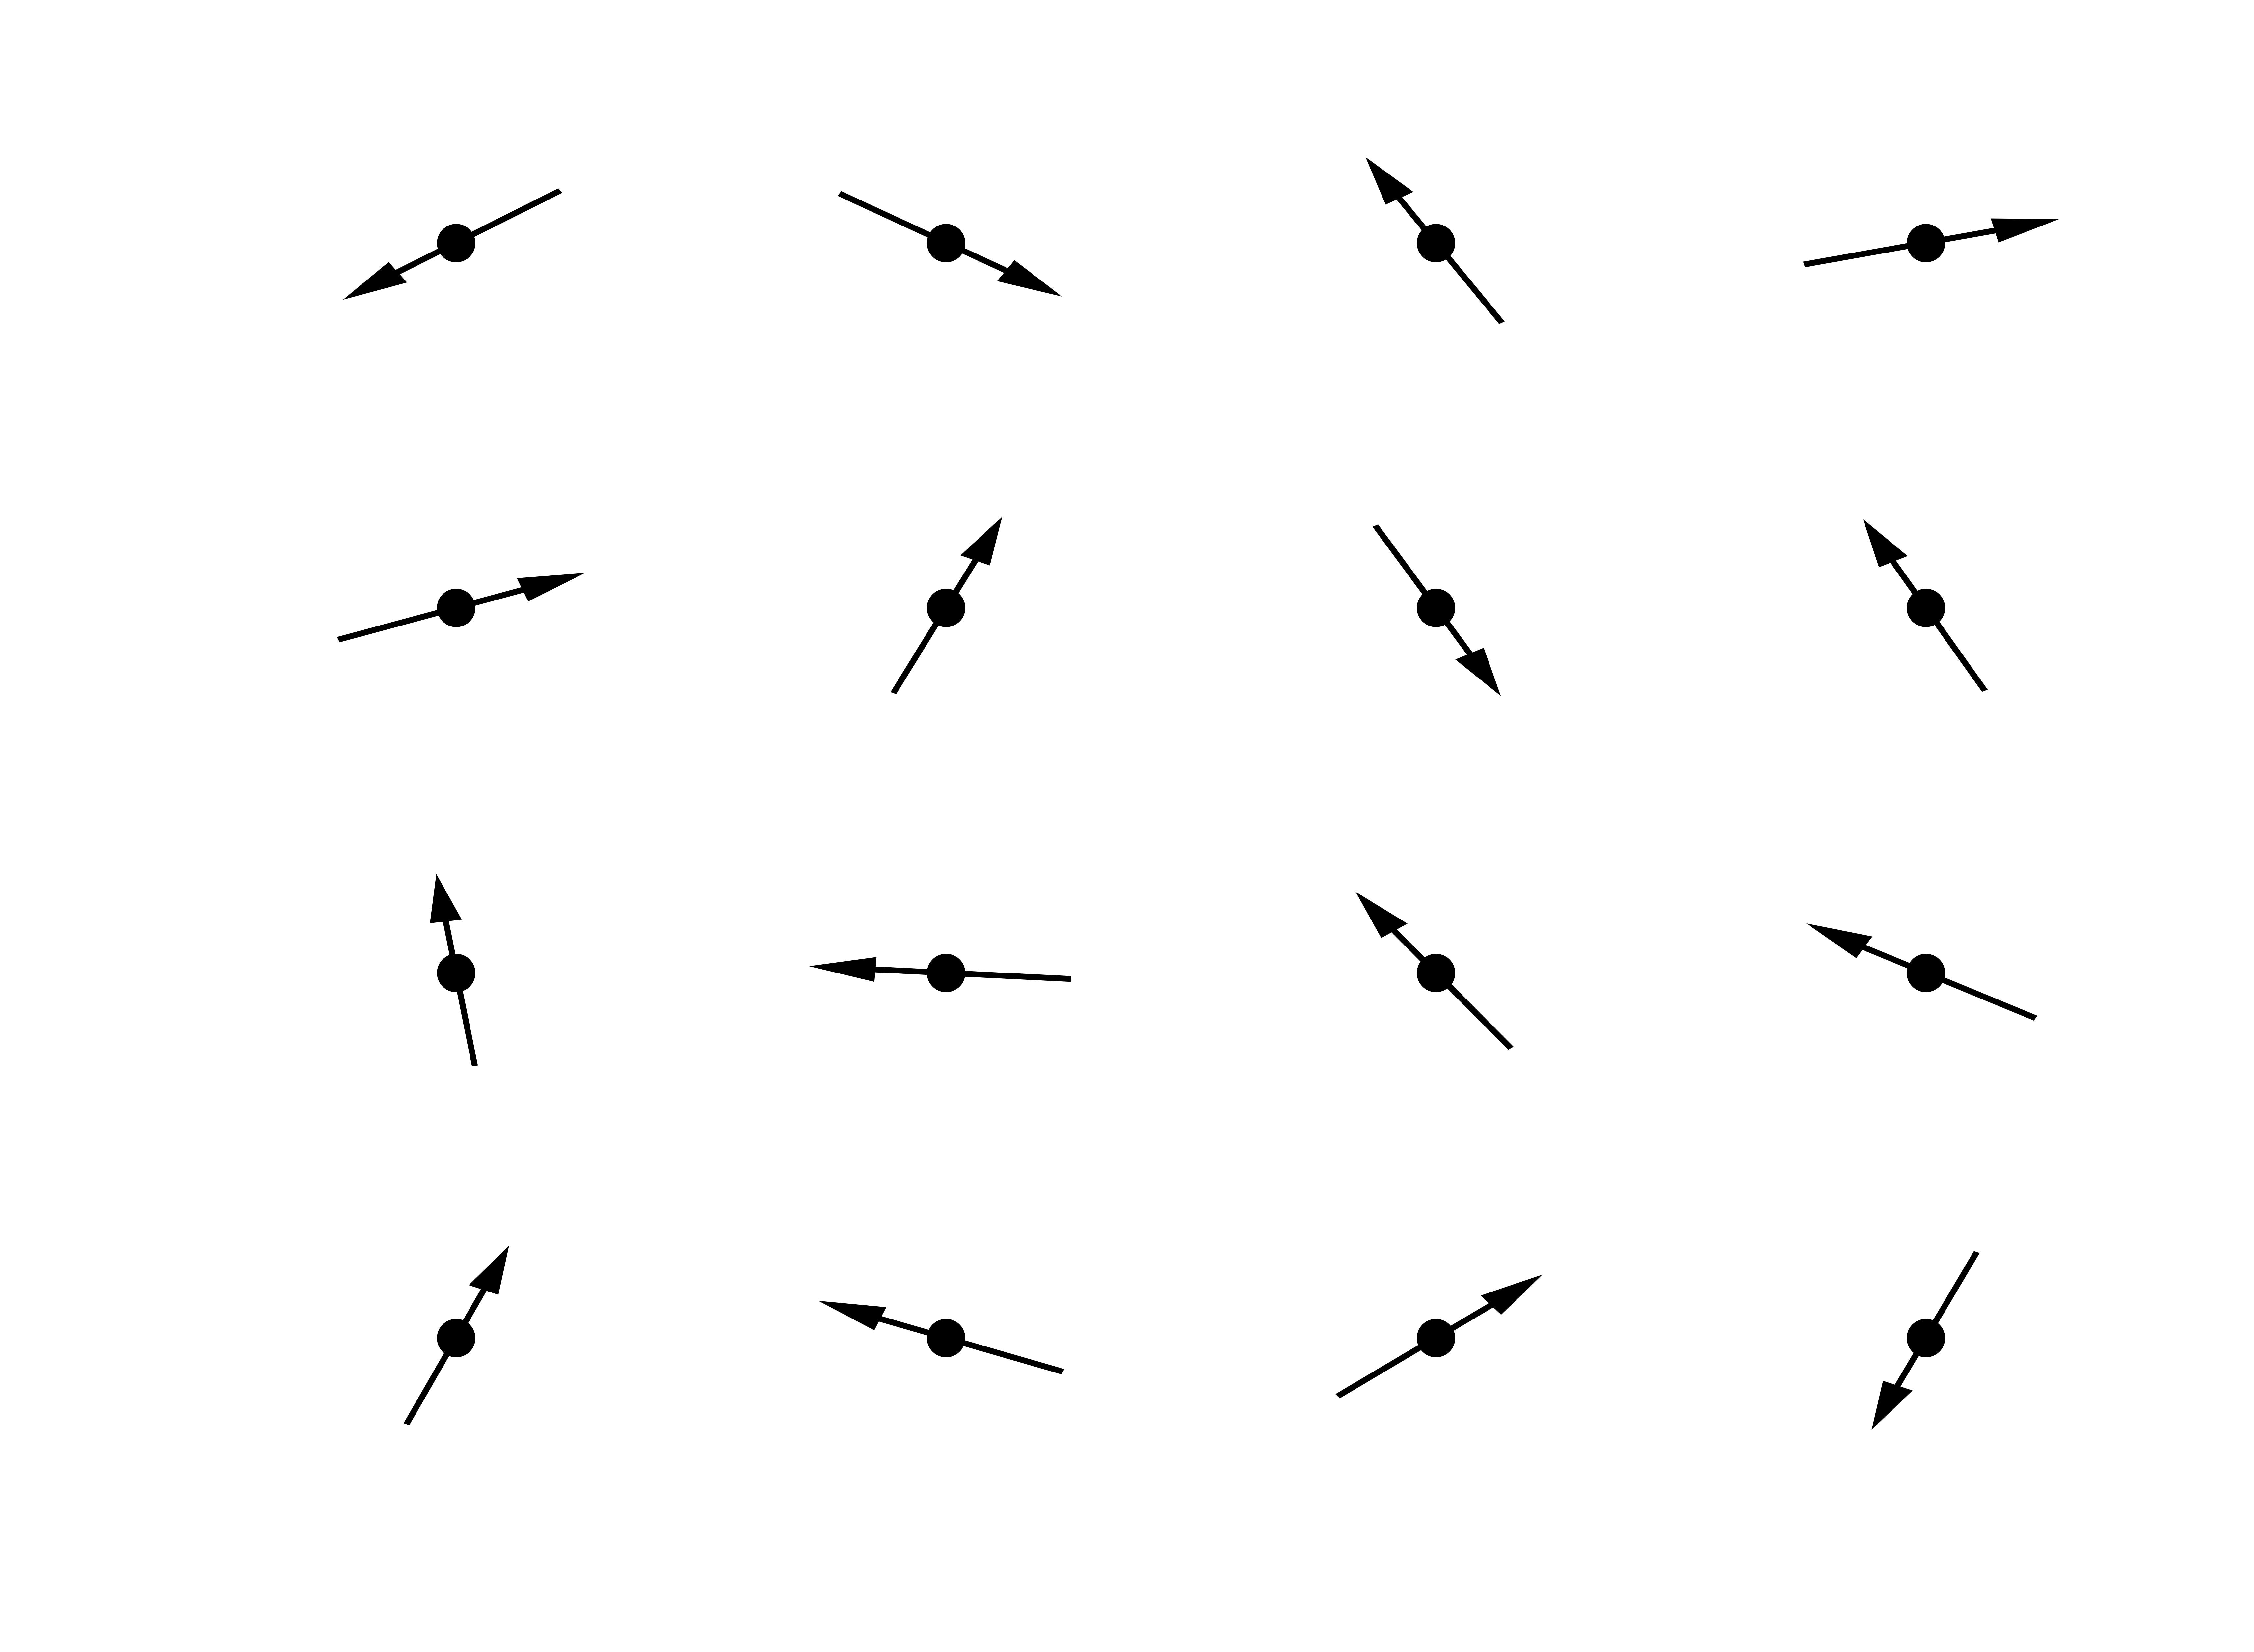
\includegraphics[width=\linewidth]{figures/randomPhaseShift.pdf}
        \caption{Higher energy state}
        \label{fig:xyhigher}
    \end{subfigure}
    \caption{A phase shift for $\mu = x$}
\label{fig:xyphaseshift}
\end{figure}

The free energy change $\Delta F$ for such a shift is

\begin{equation}
    \Delta F = L^d \cdot \frac{1}{2} \rho_s \left( \frac{A}{L} \right)^2 \Rightarrow \rho_s = \lim_{A \to 0} L^{2 - d}\frac{\partial^2 \Delta F}{\partial A^2}
\end{equation}

where $d$ is the dimension and $\rho_s$ is the superfluid density which is zero for a high energy state. The free energy is

\begin{equation}
F = - T \ln(Z) \Rightarrow F'' = T \left(\left(\frac{Z'}{Z}\right) - \left( \frac{Z''}{Z} \right)^2 \right)
\label{eq:xyfreeenergy}
\end{equation}

where $F' = \partial F / \partial A$. Examining $Z$ from Equation (\ref{eq:xypart2}) with the added shift

\begin{align}
    Z &= \prod_i \int \frac{\mathrm d \theta_i}{2 \pi} \sum_{J_{\langle ij \rangle} = -\infty}^{\infty} \prod_{b = \langle ij \rangle} I_{J_{\langle ij \rangle}} ( K ) e^{i J_{\langle ij \rangle} (\theta_i - \theta_j + \Phi_\mu)} \\
%
    & = \prod_i \sum_{J_b} \left ( \int \frac{\mathrm d \theta_i}{2 \pi} e^{i N_i (\theta_i - \theta_j)} \right ) \left ( \prod_b I_{J_b} \right ) \cdot e^{i A \frac{1}{L} \sum_i J_{i, i+\mu}} \\
\label{eq:xypart3}
\end{align}

where in the last step

\begin{align}
    \prod_i \left (\prod_{\langle ij \rangle} e^{i J_{\langle ij \rangle} \Phi_\mu} \right) &= \\
%
    \left\{ \text{$\Phi_\mu \neq 0$ only for neighbours in the $\mu$ direction} \right \} &= \\
%
    \prod_i \left ( e^{iJ_{i, i+\mu} \Phi_\mu} \right ) &= \\
%
    e^{iA \frac{1}{L} \sum_i J_{i, i+\mu}}
\end{align}

Introduce the winding number in the $\mu$ direction as

\begin{equation}
    W_\mu = \frac{1}{L} \sum_i J_{i, i+\mu}
\label{eq:defwinding}
\end{equation}

Intuitively, this describes the net flux in the $\mu$-direction. Given a loop within the bounds of the lattice, the winding number is always zero. This is since an equal amount of flux in $+\mu$ as in $-\mu$ is needed to form a loop. However, this is not the case for a percolating cluster going, for example, from $-\mu$ to $+\mu$ connecting with periodic boundary conditions. For such a `winding' cluster, the winding number will be $+1$. An example can be seen in Figure (\ref{fig:fluxpercolation}).

\begin{figure}[h!]
    \centering
        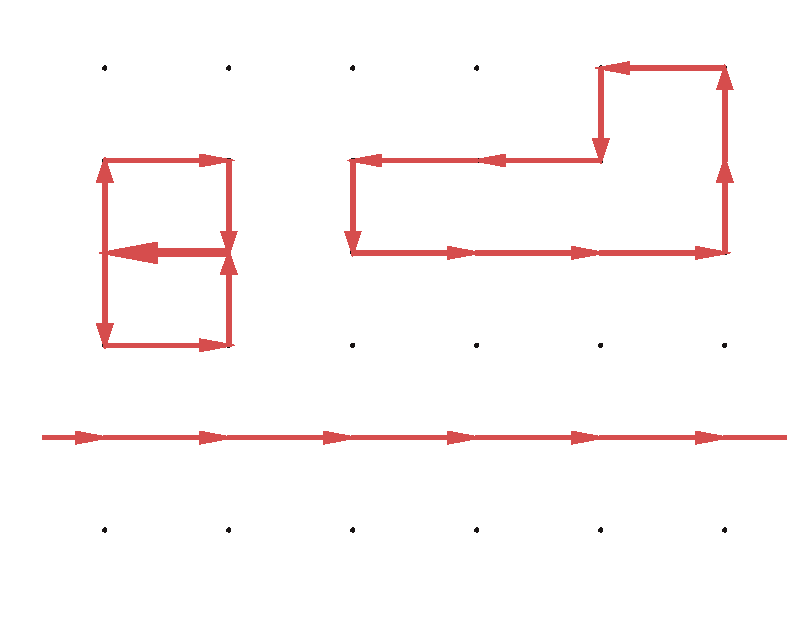
\includegraphics[width=0.8\textwidth]{figures/percolatingFlux.pdf}
    \caption{Three flux clusters on a square lattice. One percolating cluster with $W_x = +1$. The size of each arrow corresponds to the number of flux quanta between two sites.}
    \label{fig:fluxpercolation}
\end{figure}

Using the definition (\ref{eq:defwinding}) for the winding number in the partition function in Equation (\ref{eq:xypart3}) yields

\begin{align}
    Z &= \sum_{J_b} \left ( \prod_b I_{J_b} \right ) \prod_i \left ( \int \frac{\mathrm d \theta_i}{2 \pi} e^{i N_i (\theta_i - \theta_j)} \right ) \cdot e^{i A W_\mu} \\
    &= \sum_{J_b, \ N_i = 0} Z_0 \cdot e^{i A W_\mu} \\
    &= \sum_{W_\mu} Z_0 \cdot e^{i A W_\mu}
\end{align}

Using this result in Equation (\ref{eq:xyfreeenergy}) gives

\begin{align}
    \frac{\partial^2 F}{\partial A^2} &= T \left ( \left ( \frac{\sum_{W_\mu} (i W_\mu) Z_0 e^{iAW_\mu}}{\sum_{W_\mu} Z_0 e^{iAW_\mu}} \right )^2 - \frac{\sum_{W_\mu} (- W_\mu^2) Z_0 e^{iAW_\mu}}{\sum_{W_\mu} Z_0 e^{iAW_\mu}} \right ) \\
%
    &= T \left ( -\langle W_\mu \rangle^2 + \langle W_\mu^2 \rangle \right ) \\
%
    &= T \langle W_\mu^2 \rangle
\end{align}

where $\langle W_\mu \rangle = 0$ since there is an equal chance of percolating from $-\mu$ to $\mu$ as the other way around.

The superfluid density can finally be determined as

\begin{equation}
    \rho_s = L^{2 - d} T \langle W_\mu^2 \rangle 
\end{equation}

\subsection{Villain approximation}
\label{subsec:villainApprox}


In the Villain model the Hamiltonian has the form \cite{Villain:VillainOriginalPaper}

\begin{equation}    
    H = \sum_{ij} V_{ij}( \theta_i - \theta_j) + \sum_i U(\theta_i)
\end{equation}

By taking

\begin{align}
    V_{ij}( \theta_i - \theta_j) &= -J \cos ( \theta_i - \theta_j) \\
    U( \theta_i ) &= 0
\end{align}

the XY model in Equation (\ref{eq:xymodel}) is recovered.

The approximation then made by Villain was to replace the magnetic Hamiltonian one which would simplify the calculations by making the integrals Gaussian \cite{Villain:VillainOriginalPaper}.

Through a series of transformations the energy in this approximation can be written as \cite{Jos:VillainExtended}

\begin{equation}
    E = \frac{1}{2} \sum_i J_i^2
\end{equation}

where $J_i^2$ is the flux from site $i$.

The acceptance probability (see Section \ref{sec:MetropolisAlgorithm}) is therefore

\begin{align}
    A_{ab} &= \min \left ( 1, e^{-\Delta E} \right ) \\
    &= \min \left ( 1, e^{-\frac{1}{2} \Delta J_{ab}^2} \right )
\end{align}

where $J_{ab}$ is the link between site $a$ and $b$.

\subsection{Energy Scaling}
\label{subsec:xyenergyScaling}

The scaling behaviour of the heat capacity is \cite{Plischke:EqStatMech}

\begin{equation}
    C = \frac{e}{t} = \tilde a t^{-\alpha} + \tilde b
\end{equation}

where $t = |T - T_c|$, $\alpha = -0.01$, and $\tilde a, \ \tilde b$ are some constants.

Therefore, the energy per site, $e$ is

\begin{equation}
    e = a t^{1 - \alpha} + b
\end{equation}

And the total energy

\begin{equation}
    E = L^d ( a t^{1 - \alpha} + b ) \propto L^d, \ \text{at $T = T_c$}
\end{equation}

where $d$ is the dimension of the sample. This scaling behaviour for the total energy can be seen in Figure (\ref{fig:results_energyxy}) for $d = 3$.

\section{Hausdorff dimension}
\label{sec:hausdorffdimension}


Let $X$ be a metric space, $\alpha$ be some positive real number, then the $\alpha$-Hausdorff measure of a subset $A \subset X$ is defined as 

\begin{equation}
    \mathcal{H}^{\delta}_\alpha (A) = \inf \left \{ \sum_{B \in \mathcal{B}} \left ( \text{diam}(B) \right)^\alpha \right \}
\end{equation}

where $\mathcal{B}$ is a cover of $A$ of closed balls with diameter no larger than $\delta$ \cite{Heinonen:HausdorffDimMath}.

Taking the limit where $\delta \to 0$, the number of possible covers decreases. Since the limit is bounded from below, the limit exists \cite{Rudin:PrincMathAnalysis} and

\begin{equation}
    \lim_{\delta \to 0} \mathcal{H}^{\delta}_{\alpha} (A) = \mathcal{H}_\alpha (A) \in [0, \infty )
\label{eq:hausdorffmeasure}
\end{equation}

Examining Equation (\ref{eq:hausdorffmeasure}) gives

\begin{align}
    \lim_{\delta \to 0} \mathcal{H}^{\delta}_{\alpha} (A) &= \lim_{\delta \to 0} \inf \left \{ \sum_{B \in \mathcal{B}} \left ( \text{diam}(B) \right)^\alpha \right \} \\
%
    &\leq \lim_{\delta \to 0} \inf \left \{ \sum_{B \in \mathcal{B}} \delta^\alpha \right \} \\
%
    &= \lim_{\delta \to 0} \inf \left \{ N_{\delta}^A \delta^\alpha \right \}
\end{align}

where $N_{\delta}^A$ is the number of balls with diameter $\delta$ that can cover $A$. Though not a proof, one can intuitively say that if for some $\alpha > 0$ the limit is finite, then $\mathcal{H}_{\alpha'} = 0$ for each $\alpha' > \alpha$. Therefore the number

\begin{equation}
    \text{dim}_H (A) = \inf \{ \alpha > 0 : \mathcal{H}_\alpha (A) = 0 \}
\end{equation}

exists and is called the Hausdorff dimension of $A$ \cite{Heinonen:HausdorffDimMath}.


\section{Box dimension}
\label{sec:boxdimension}

Given some subset $A$ of a metric space $X$, let $N(\epsilon)$ be the number of boxes with side length $\epsilon$ needed to cover $A$. Then the box dimension $d$ of $A$ is defined as \cite{strogatz:dynamics_chaos}

\begin{equation}
    d = \lim_{\epsilon \to 0} \frac{\ln N(\epsilon)}{\ln 1 / \epsilon}
\end{equation}

if the limit exists.

For intuition it helps to look at some examples. If $A$ is a smooth line of length $l$, then the number of boxes needed to cover $A$ scales as

\begin{equation}
    N_l(\epsilon) \propto \frac{L}{\epsilon}
\end{equation}

while for some two dimensional region with area $\Lambda$ the boxes needed is

\begin{equation}
    N_{\Lambda}(\epsilon) \propto \frac{\Lambda}{\epsilon^2}
\end{equation}

such that for a $d$-dimensional subset $A$, the boxes needed will scale as

\begin{equation}
    N (\epsilon) \propto \frac{1}{\epsilon^d} \Rightarrow d = \frac{\ln N(\epsilon)}{\ln 1 / \epsilon}
\end{equation}

Note that the box dimension and the Hausdorff dimension coincides for fractals that satisfy the open set condition \cite{Falconer:RelHausdorffBox}.

The open set condition says that for a sequence of contractions $c_1, c_2, ..., c_m$ exists a nonempty open set $V$ such that \cite{Bandt:OSC}

\begin{equation}
    \cup_{i = 1}^m c_i(V) \subset V, \ \text{and} \ c_i(V) \cap c_j(V) = \emptyset \ \text{for} \ i \neq j
\end{equation}

Intuitively, this means that the images $c_i(V)$ do not overlap `too much'.

\subsection{Scaling Dimension}
\label{subsec:ScalingDimension}

Another way of determining the Hausdorff dimension is to consider a scaling system \cite{Camarda:MethodsDetermineHausdorff}. The scaling behaviour of the largest cluster should then follow

\begin{equation}
    N = L^{D_H}
\end{equation}

where $N$ is the number of links in the largest cluster, $L$ is the linear system length and $D_H$ is the Hausdorff dimension.

This scaling relation can be seen in Figure (\ref{fig:results_maxloopdimension}).


